% Chapter 1

\chapter{Introduction} % Main chapter title

\label{Chapter1} % For referencing the chapter elsewhere, use \ref{Chapter1} 

%----------------------------------------------------------------------------------------

% Define some commands to keep the formatting separated from the content 
\newcommand{\keyword}[1]{\textbf{#1}}
\newcommand{\tabhead}[1]{\textbf{#1}}
\newcommand{\code}[1]{\texttt{#1}}
\newcommand{\option}[1]{\texttt{\itshape#1}}

%----------------------------------------------------------------------------------------
\section{Autonomy and decentralization in satellite systems}

%1) Actualmente se estan estudiando nuevos conceptos y arquitecturas de misión: las misiones distribuidas.
In the context of satellite missions, new mission architectures and original approaches are currently being explored. Traditional monolithic satellites are being replaced by decentralized satellite architectures, such as fractionated spacecraft or satellite swarms.

Miniaturization of technology, reduced launch costs, and standardization are increasing the interest in small satellites for these \textbf{distributed missions}. These small satellites are satellites of reduced size and low mass (under 500 kg). They can be classified according to its mass in: \emph{small-satellites} from 500 kg to 100 kg, \emph{micro-satellites} 
from 100 kg to 10 kg, \emph{nano-satellites} from 10 kg to 1 kg, \emph{pico-satellites} from 1 kg to 100 g and \emph{femto-satellites} for less than 100 g. With clusters of these smaller modules, distributed missions are aimed at serving Earth Observation requests with similar or better characteristics (e.g. spatial resolution, revisit time) than those of large monolithic satellite systems, while reducing their cost and development times. 

They are also seen as a feasible alternative to achieve better spatial resolutions and shorter revisit times. In fact, the requirements of future Earth Observation applications (e.g. real-time video, stereoscopic radar, multi-spectral imagery) might only be cost- and time-effective through the implementation of these new mission approaches, where several small units work cooperatively to acquire data.

Moreover, the fractionation of satellites and their decentralization allows the system to continue operating even when some of its parts is malfunctioning, something that increases the robustness and reliability of the system.

%2) Aunque es un ámbito nuevo que aún está en vías de exploración, este contexto exige el estudio de sistemas de gestión para tales misiones.
%3) Los sistemas de gestión tradicionales para satélites se basan en planificadores complejos y centralizados que se ejecutan en el segmento de Tierra.
Despite the fact that distributed mission are still being explored, this context requires the study of management systems capable to govern these complex systems. Traditional management systems are mainly based on centralized complex planners that run on the ground station, but this approach does not benefit from all the advantages of the distributed satellite system. For this reason, the management systems for distributed satellite missions under research tend to be decentralized.

%4) Paralelamente, hay un paradigma que cada día se extiende más: proveer de autonomía a las naves (spacecraft).
Simultaneously, the research on satellite missions is also becoming more and more focused on a new paradigm in the satellite's conception: to provide increasing \textbf{autonomy} to the spacecraft.
%5) La autonomía se prevé necesaria, sobretodo, por los siguientes motivos:
%	5.a) Para ganar en resiliencia (y por tanto mejorar la robusteza de la misión).
%	5.b) Para mejorar el performance de la misión mediante el análisis de datos a bordo, que permiten ajustar mejor los instrumentos y centrarse en puntos de mayor interés (sin tener que pasar por Tierra y perder tiempo, y en consecuencia sin perder oportunidades de observación).
%	5.c) En misiones distribuidas con muchos nodos conectados, en los que mantener el control centralizado es inviable.
Some benefits of having autonomous spacecraft are:
\begin{itemize}
\item To provide a better resilience to the system (e.g., it does not depend on other entity and the state of the communication channel in between), which will increase the robustness of the whole mission.
\item To improve the mission's performance through on-board data analysis. This allows to adjust on-board instruments and focus on higher interest locations or events without transmitting the data to ground and waiting for instructions.
\item To enable huge distributed systems with many interconnected nodes to decentralize the management, as in these cases a centralized operation would be unfeasible.
\end{itemize}

%6) Autonomía + Misiones distribuidas = se requiere explorar nuevos sistemas de planificación (Mission Planning Systems), que sean distribuidos y que se ejecuten on-board (dos puntos clave).
%7) El objetivo es proveer de autonomía a la constelación y solucionar el problema de gestión.
%%%%Aquí m'he quedau 002143T24012016
%This sentence makes me understand that "autonomy" and "distribution" are things or features that I can decide to put on a system or not. That's not right. These are current TRENDS and are motivated by the requirements of new Earth Observation applications ("better, cheaper, faster", better resolution, shorter revisit times, etc.)
%On the other hand, you are forgetting what a FULLY fractionated spacecraft is: a satellite decomposed into several physically-detached modules (energy system, communications, storage module, data processing module, etc.) orbiting closer and exchanging system resources (power, data, ...).
%These novel architectures have also inspired new concepts, such as "Federated Satellite Systems" in which the spacecraft opportunistically share their commodities with others in order to satisfy the needs of a global request (at the constellation level).

The autonomy and decentralization are current trends on the design of satellite missions, motivated by the requirements of new Earth Observation applications (e.g., better image resolution, shorter revisit times, etc.). Several novel mission architectures based on these concepts have appeared \citep{Araguz15,d2012distributed}:
\begin{itemize}

\item \textbf{Fully-fractionated spacecraft}: a satellite decomposed into several physically-detached modules (i.e., energy system, communications, storage module, data processing module, etc.) orbiting closer and exchanging system resources (e.g., power and data).

\item \textbf{Satellite swarms}: distributed missions in which the infrastructure nodes are independent satellites that perform their own tasks without resource exchange or collaboration. This type of distributed satellite tends to be composed of homogeneous modules with similar or identical capabilities.

\item \textbf{Trains or constellations}: group of sparsely distributed satellites with coordinated maximum ground coverage, for applications such as Earth-Observation, communication or geo-location (GPS).

\item \textbf{Federated Satellite Systems}: purely collaborative missions in which the spacecraft opportunistically share their commodities with others in order to satisfy the needs of a global request (at the constellation level) \cite{golkar2013federated}.

\item \textbf{Hybrid missions}: heterogeneous missions which combines characteristics of more than one of the presented archetypes, as they represent theoretical extremes.

\end{itemize}

These complex architectures have led to the exploration of adapted Mission Planning Systems (MPS), requiring them to be \textbf{distributed} and \textbf{executed on-board}. These MPSs aim at providing the needed autonomy to the constellation and solving the spacecraft management problem.

%8) Eso conlleva la definición de políticas de planificación diferentes, como la que se propone para ABS. 
%9) Además, la política L-G de ABS tiene en cuenta la importancia que tienen (y tendrán en el futuro inmediato) las arquitecturas basadas en nano-satélite, en las que las capacidades computacionales se ven reducidas debido a las restricciones de potencia.
%11) La política L-G, simplemente plantea desmenuzar un problema complejo en multiples pequeños más simples (analogía: la predicción meteorológica se basa en múltiples modelos locales y un macro modelo global que los "pega" y aporta coherencia en los contornos).
In this context, different Mission Planning Systems and policies have been proposed. One of these policies is the one that has been presented for the Android Beyond the Stratosphere (ABS) project,\footnote{\emph{Universitat Polit\`ecnica de Catalunya}'s (UPC) ABS project, in which context this thesis has been developed, aims at developing a nano-satellite platform standing on modular, low-cost open-source components and standards with an Android-based satellite-on-a-phone architecture.} the Local-Global policy \cite{Araguz15}.

A peculiarity of this approach is that it focuses on the nano-satellite based fractionated spacecrafts, taking into account the importance they have as the next-generation satellite missions architectures. A big challenge present in these class of space systems is that the computational capacities are reduced due to the existing power restrictions, something considered in this policy's design.

The required computational efficiency can be achieved by a partition of the scheduling problem in several simpler sub-problems such that each satellite is able to solve one of them (this could be compared to what is done for meteorology predictions, in which a number of local models are combined within a global macro-model).

%10) Tu trabajo se centra en explorar el sistema de autonomía basado en la política L-G.
The main aim of this thesis is to explore and assess a satellite autonomy system which applies the Local-Global policy, by designing, implementing and comparing it with a state-of-the-art distributed scheduling algorithm to determine whether it performs good at solving the problems it has been designed for.

First, the Local-Global policy and other state-of-the-art planning algorithms will be presented, and the details of the implementation of the two compared algorithms will be explored. Then, a benchmark for the comparison will be designed, and metrics for the experimental measures will be defined.

%--------------------------------------------------------------------------------------------------
%A scheduling algorithm is a type of optimization problem consisting on distributing tasks over a determined time window (and maybe also among a number of workers, although there could be only one) while satisfying some resource or time requirements, such as task deadlines or processing resources in the worker. In our case, we are studying a particular task scheduler which has the particularity of being \emph{distributed}: this means that in this case the scheduling problem is not solved by a sole machine but by a group of them.
%--------------------------------------------------------------------------------------------------

The most important desired result is to conclude whether the ABS policy behaves well in a simulated environment compared to other algorithms. By \emph{behaving well} it is meant that, for the defined metrics, it achieves to schedule the tasks among the workers within a minimum time and using an optimal allocation of resources.

In order to accomplish this goal the algorithms have been tested with a benchmark of multiple simulated scheduling problems. The experimental results analysis are shown at the end of the present document, before concluding and stating the future work to be done.
%--------------------------------------------------------------------------------------------------

\section{The Android Beyond the Stratosphere Project}

This thesis has been carried out in the context of the Android Beyond the Stratosphere project. This project, performed at the Nano-Satellite and Payload Laboratory of the Technical University of Catalonia -- UPC BarcelonaTech, aims at designing a standardized modular open-source nano-satellite platform based on commercial components and open standards. The satellite-on-a-phone architecture is being explored to implement a low-cost nano-satellite based on a well-known system such as Android.

Moreover, it is intended to develop a fully distributed system in which a number of these low-capacity Android-based satellites interact and collaborate to achieve global targets. The needed synchronization for this collaborative satellite constellation, as it has been stated in the previous section, requires an advanced scheduler algorithm that allows the system to distribute the tasks among all the satellites forming the system in a balanced and optimal way (in terms of time and resource consumption). This task scheduler is the core of this thesis, which is intended to design, implement and compare it with other state-of-the-art distributed task allocator, and experimentally test its efficiency and optimality.

A centralized scheduler running in a \emph{leader} satellite could be a possible solution, but the complexity of the problem and the low computational capabilities of these low-cost nano-satellites make this approach unfeasible. Although much more challenging, this type of distributed approaches provide autonomous decision capabilities to the satellites in a constellation and greatly improve the qualities of the system. Adaptiveness and low resource consumption: these are the key concepts in a system like this. With a distributed algorithm running on every satellite the computational load is shared among all and the autonomy of each satellite is preserved.
%----------------------------------------------------------------------------------------

\section{Scheduling tasks: a hard optimization problem}

%A scheduling algorithm is a type of optimization problem consisting on distributing tasks over a determined time window (and maybe also among a number of workers, although there could be only one) while satisfying some resource or time requirements, such as task deadlines or processing resources in the worker. In our case, we are studying a particular task scheduler which has the particularity of being \emph{distributed}: this means that in this case the scheduling problem is not solved by a sole machine but by a group of them.

The core of this thesis is a typical optimization problem: to schedule some input tasks with varying or fixed processing time taking into account the resources available in the system and the time requirements that the tasks may have, such as different arrival times, deadlines or dependence between tasks.
%to schedule some input tasks over a determined time window (and maybe also among several workers) while satisfying some resource or time requirements, such as task deadlines or processing capabilities in the worker. In this case, the task scheduler under study has the particularity of being \emph{distributed}: this means that the scheduling problem is not solved by a sole machine but by a group of them.

Scheduling becomes a hard problem that has to be solved with advanced programming techniques such as constraint-based programming or heuristics. In fact, most problems, such as multiprocessor scheduling or Job Shop Scheduling, are proven to be NP-hard optimization problems.

%--------------------------------------------------------------------------------------------------
%The problem that our algorithm must solve can be reduced to a multiprocessor scheduling problem (so it can be demonstrated it is a NP-hard problem): given a set \emph{A} of jobs where job $a_i$ has a processing time equal to $l^{a_{i}}$, arrives to the system at $t_0^{a_i}$ and has to be finished before the deadline $t_{\text{max}}^{a_i}$, and a set of workers \emph{W}, which is the optimal schedule of the maximum of jobs such that all resource and time requirements are accomplished? The optimality here can be described as a set of attributes of the solution that are chosen for a particular problem. In the algorithm description section we will explain the parameters that we have chosen as \emph{optimality testers}.
%--------------------------------------------------------------------------------------------------

This problem has been studied deeply (in fact it is a very mature field of research), and there are many well-known scheduler algorithms for one or many workers (e.g., EDD, EDF, RM… \cite{leung2004handbook}). However, they are mainly mono-processor algorithms, i.e. the algorithm runs in a single machine and if the solution applies to other machines, it is sent to them. The recent growth of distributed systems with increasing autonomy and processing capacity, very present in the IoT, WSNs (Wireless Sensor Networks) and robotics, has led to accelerate the research on distributed schedulers. 

This last case applies to this work: The nodes have to cooperatively solve an NP-hard problem, i.e. the satellites executing the algorithm must achieve a solution which is good for all the system by only knowing its own state and communicating with the others to agree the final solution. Moreover, the nodes are working with heavily constrained inter-satellite communication channels. It can be easily concluded that \emph{distributing} a task scheduler adds much complexity to an already computationally hard problem. But this is not necessarily true: one of the most widely used computer science paradigms is ``divide and conquer''. The advantages of sharing the computational burden clearly outweigh the communication costs. 

%----------------------------------------------------------------------------------------

\section{Distributed systems}

%The objective of this section is twofold: to have a basic knowledge of what is and what is not a distributed system and to describe the characteristics of distributed programming that make it quite different from typical mono-processor programming. This is important as long as this Thesis' core is a \emph{distributed} algorithm for a \emph{distributed} system.
%
Distributed systems are formally defined in \cite{Coulouris:2011:DSC:2029110} as \textit{``software systems in which components located on networked computers communicate and coordinate their actions by passing messages''}. Therefore, the basis of these type of software systems is the communication. By \emph{talking} with the other workers in the network a component of the system can take into account the shared knowledge about the state of the rest of nodes and work to obtain the whole system's goal.

There are multiple architecture designs available for distributed systems, having both \textbf{centralized} and \textbf{fully-independent} structures \cite[p.~36]{Tanenbaum:2006:DSP:1202502}. Sometimes it is needed to have a single node doing some special functions to control the state of the entire system\footnote{In fact, leader election and recovery is one of the most critical functionalities in distributed programming.}. However, it means always a single point-of-failure, a weakness that affects the robustness of the entire system, apart from decreasing the system throughput whenever it is needed to contact the leader, which can be a bottleneck. This does not mean that in some situations the presence of a \emph{master} node is a strength for the system, because it itself is a high-capacity robust node (e.g., consider the ground station of a satellite constellation).

\subsection{Distributed mission planners}
 
%Distributed algorithms are not just a sequential single-processor code that has been decomposed into several pieces and assigned to a number of processors.
Distributed algorithms are pieces of code designed to run on several nodes, having as a key function the intercommunication between nodes.

The autonomy of the nodes running the distributed planners modifies some typical programming patterns. Also synchronism problems or node failures appear. These new challenges are solved with different approaches: problem's solution achieved by \emph{consensus} among nodes, clock synchronization algorithms, data consistency and reliable communication, redundancy and failure recovery... \citep{Tanenbaum:2006:DSP:1202502}

The present thesis will not focus on the synchronism and failures problems, but on the ability of distributing computational efforts to solve a complex scheduling problem. This will be key to improve the computational efficiency of the system: how it takes profit of the intercommunication to precisely distribute the work without missing crucial information for obtaining the optimal scheduler.
%----------------------------------------------------------------------------------------

\section{Previous work}
\label{sec_previouswork}
ABS project has been developed for two years and a half, and a prototype of an individual Android-based satellite is being finished, with some work in hardware integration still to be done. The distributed software architecture is also a key part of this project: it is intended to be as generic as possible, in order to enable the deployment of any distributed satellite system topology.

The task scheduler is a key part of this distributed architecture, as it enables the whole system to achieve the global goal while distributing smaller tasks among all the nodes composing the constellation.

\subsection{The Local-Global policy}

In \citep{Araguz15} the main characteristics of the distributed task scheduler proposed for the ABS project were described, and its procedure completely explained. However, an implementation was to be done and there were still no experimental results to be shown. In this thesis this policy has been fully designed and implemented, and experimental measures have been taken through a benchmark specifically designed. Below a brief description of the presented algorithm is shown.

This scheduling policy aims at providing an adaptive technique for a distributed spacecraft to find an optimal schedule for an arbitrary number of satellites composing it. To be capable of modelling the possible heterogeneity present among the different nodes, this algorithm takes into account the processing capabilities and available resources of every node.

The policy basically divides the multi-ple\hskip0pt-\hskip0pt tasks multiple-workers problem into several multiple-tasks single-worker sub-problems. Every \emph{Local} entity (i.e. every system node) will evaluate each sub-problem, as if it was a fully-local scheduling problem, and the solutions found locally are sent to the \emph{Global} layer, represented by a master node, which will be in charge of combining them and finding out the optimal schedule. Once the final solution is generated, the \emph{Global} node sends it to the rest of the constellation.

\begin{figure}[h!]
\centering
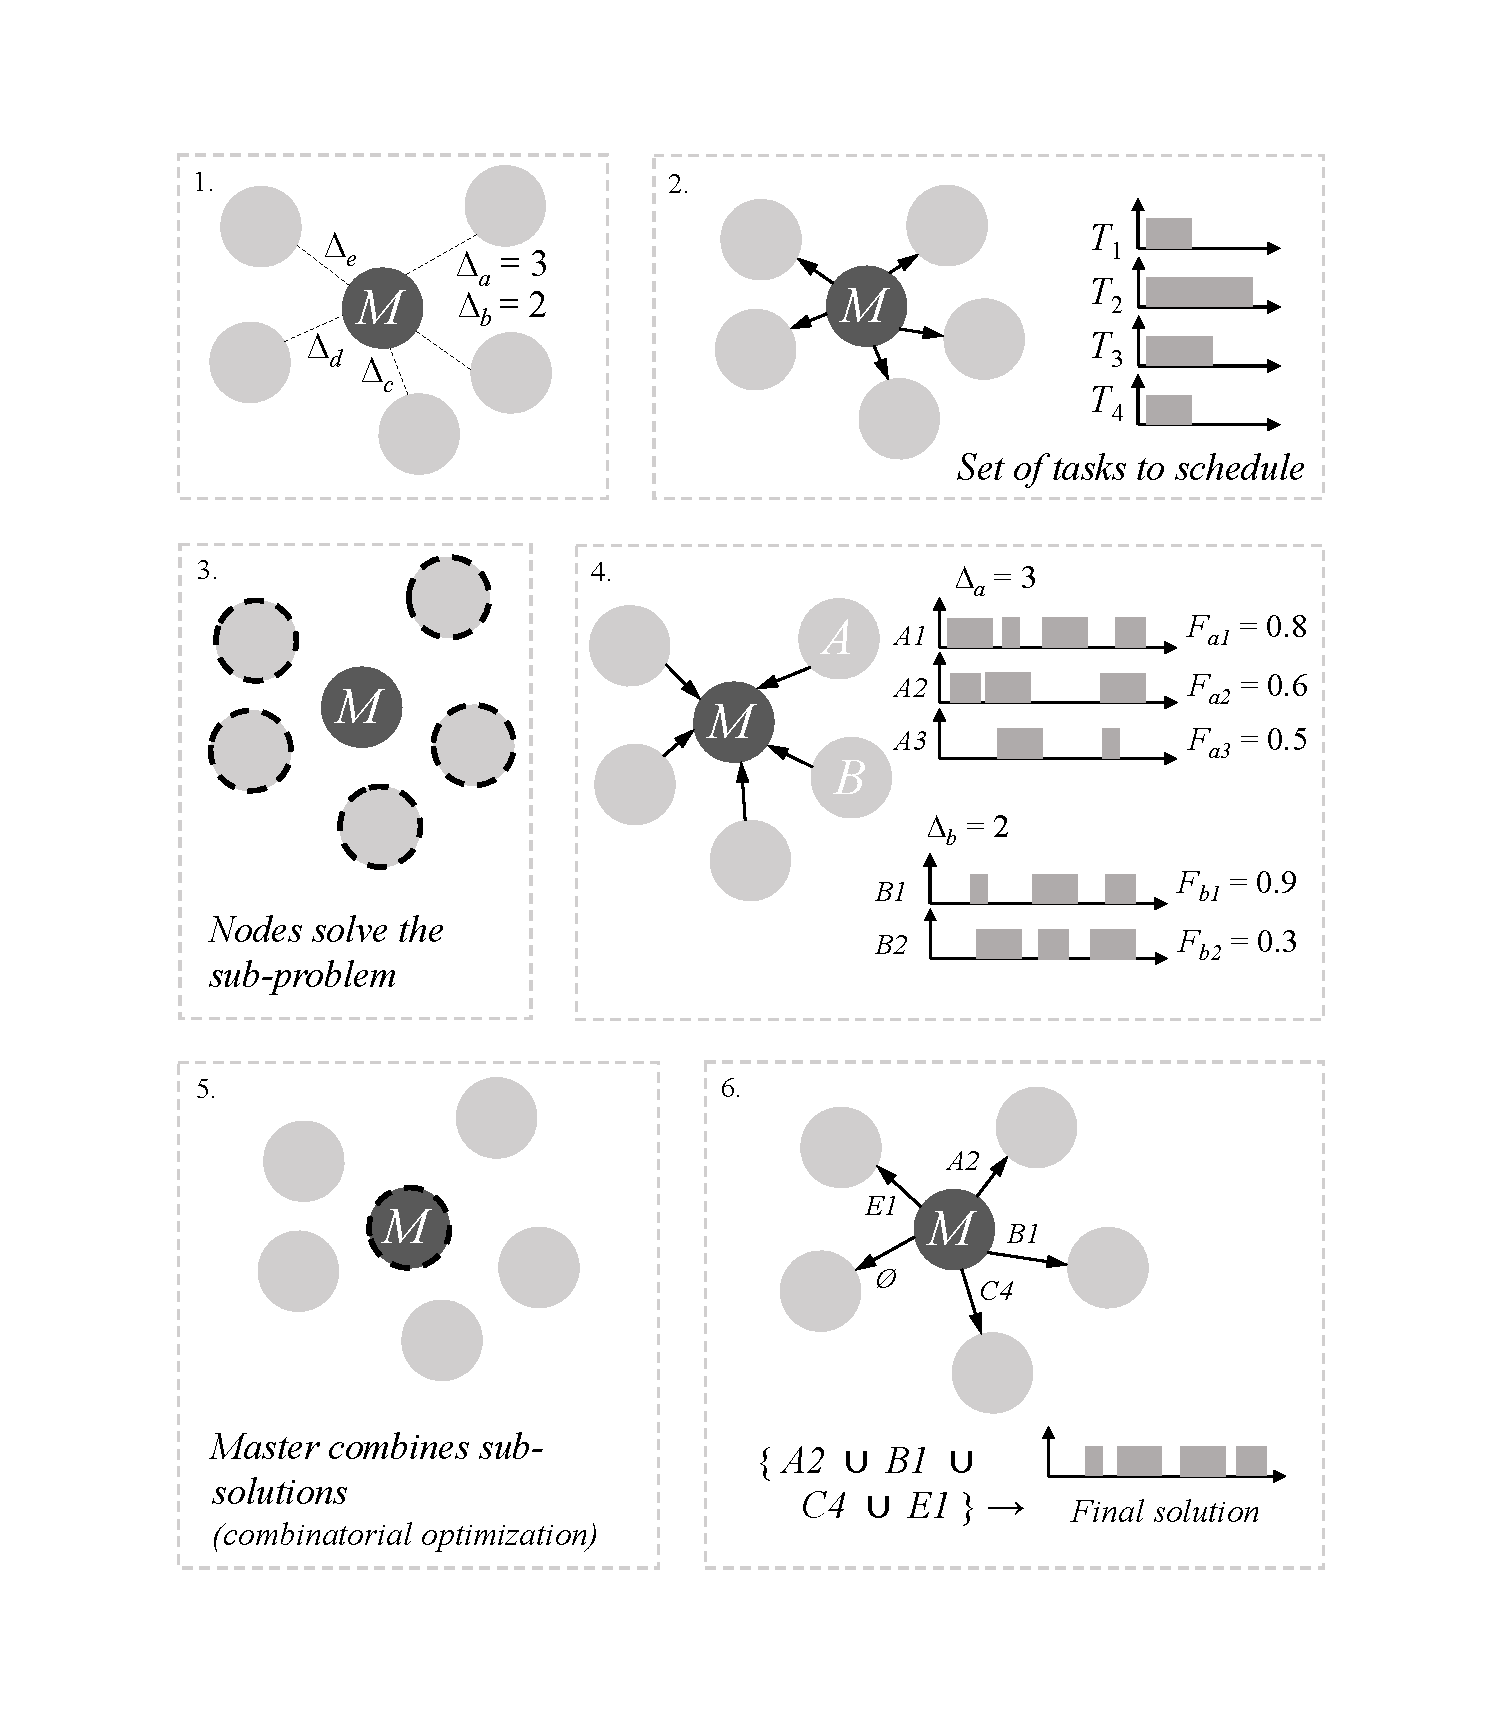
\includegraphics[scale=0.3]{Figures/figure_policy_steps.pdf} 
\caption{Local-Global policy steps (as extracted from \cite{Araguz15})}
\label{fig_LGsteps}
\end{figure}

To make possible the re-composition of the initial problem and to enable the master to find out the optimal combination taking into account as much information of the \emph{quality} of each local solution as possible, two parameters are defined: the figure of merit \emph{F} and the golden index $\Delta$. The first of these parameters measures the goodness of each local solution, as a set of parameters describing it. The second one is the number of possible solutions that each \emph{Local} entity can report to the global layer, and is meant to balance the potential heterogeneity in the system: nodes possessing higher processing capabilities will obtain a higher $\Delta$ than those with lower computational resources.

Having described the basics of the Local-Global algorithm the procedure it follows will be now divided in six steps (see also Fig. \ref{fig_LGsteps}):

\begin{enumerate}
\item \textbf{Characterization.} The $ \Delta $ value for each satellite is assigned, after considering its computing capabilities.
\item \textbf{Task delivery.} Master node selects the time window (duration of the schedule to be produced by the scheduling algorithm) and discards the tasks that cannot be scheduled \emph{a priori}. After this, it sends to every \emph{Local} entity the set of tasks, so that they can begin to compute sub-solutions.
\item \textbf{Local evaluation.} Local entities' task planners produce as many solutions as its $ \Delta_i $ value, attaching to each sub-solution an \emph{F} value.
\item \textbf{Submission of solutions.} Each satellite provides the set of at most $ \Delta_i $ solutions, sending for each one the list of tasks included in that schedule solution and its figure of merit \emph{F}.
\item \textbf{Global selection and combination.} The master triggers a combinatorial optimization process that selects at most one sub-solution per satellite in order to maximize the aggregated \emph{F} value, which is not necessarily the sum of the single \emph{F} values.
\item \textbf{Distribution of solution.} The master notifies each \emph{Local} entity with the identity of its selected sub-solution, if any.
\end{enumerate}

In section \ref{LGimplementation} the focus will be on the implementation that has been developed in this thesis, specifying the \emph{Local} entity task planner characteristics and the optimization algorithm used in the global layer.